\section{Our \ApproachName{} Approach} 
\label{sec:Approach}

This section explains how our \ApproachName{} approach makes use of evolutionary computation to transplant organs within video games content. We first present an overview of our approach and subsequently provide the details of the approach. To help the reader, we provide along with the approach explanation an example of transplantation of content within a simplified version of \sq{bosses} of the video game \CaseStudy{}.

Fig.~\ref{fig:approach} shows an overview of our approach.
At the top left of the figure we show the input to our approach, which are the organ to be transplanted from the donor and the host where the organ will be transplanted. Afterwards, \ApproachName{} detects the points of the organ that allows the transplantation and the points where the organ can be inserted into the host. To initialize the population of the evolutionary algorithm, the organ is cloned and transplanted in a random point. Genetic operations generate potential solutions for transplantation, while the objective function asses the quality of these solutions. This process of generating and assessing is repeated until a specific stop condition is met. When the evolutionary algorithm finish the execution we obtain a ranked list by the objective function of the best transplantation between organ and host.

In video games, software models are popular (compared to classic software) possibly because they facilitate the participation of non-programmers (e.g. artists) in the development process. Therefore, our \ApproachName{} approach is designed to work with models. Although we illustrate the running example with the SDML models of the case study, our approach is generic and can be used with other modelling languages because it exploits the idea of boundaries between model elements.
Next, we describe each step of \ApproachName{} in the following subsections.

\begin{figure}[h]
    \centering
    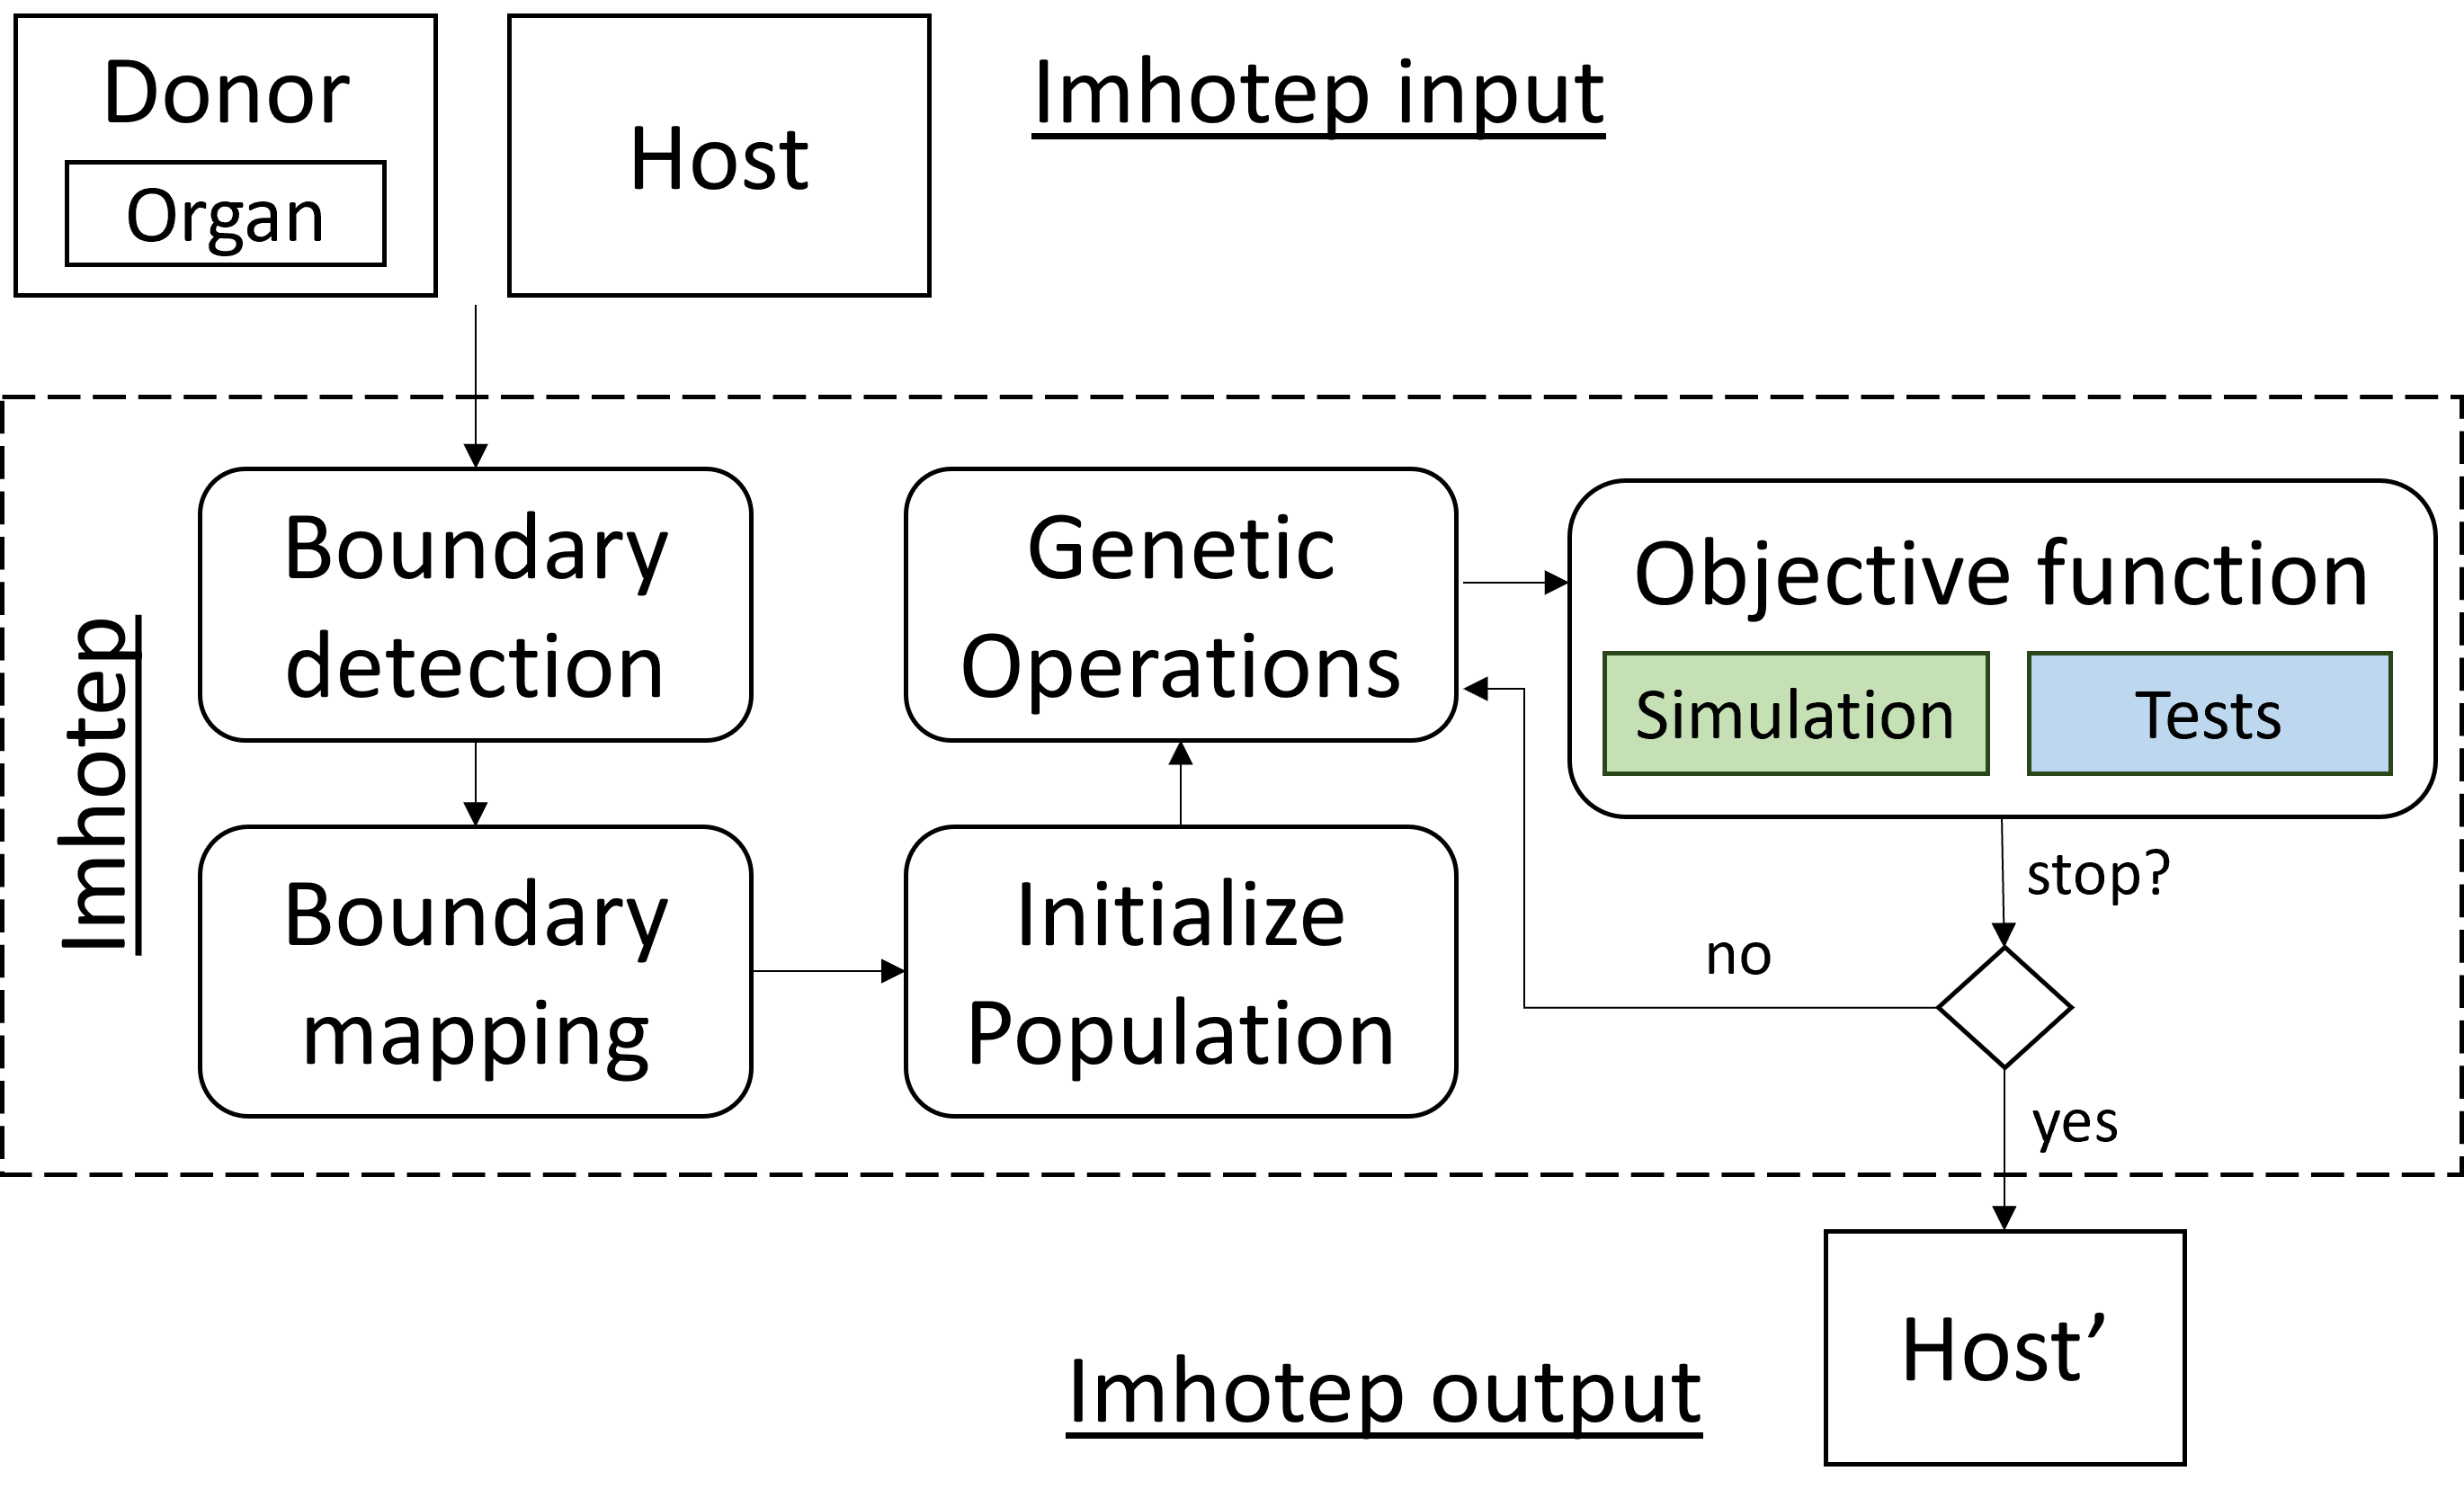
\includegraphics[width=0.45\textwidth]{Figures/overview.png}
    \caption{Overview of our \ApproachName{} approach.}
    \label{fig:approach}
\end{figure}


\subsection{Input selection}

\ApproachName{} requires the developers to identify a source model content (donor) with the organ that will be transplanted, and a target model content (host). %The models used in \ApproachName{} are models based on SDML as explained in the background section (\ref{sec:Background}). The donor and host from the example are a simplified version of the donor and host used in the evaluation, which we think they will help to understand the approach.
In our running example we present a simplified version of the metamodel, and the corresponding concrete syntax of the model (see Fig.~\ref{fig:metamodel+syntax}) from the video game \CaseStudy{}. 
\sq{Hulls} serve as the structural framework that define the anatomical composition of the models. For example, the boss presented on Fig.~\ref{fig:scenario} (identified as \sq{B}) has its body built by hulls.
\sq{Weak points} points are conceptual elements that possess the vulnerability to be harmed.
\sq{Weapons} are tangible items capable of causing harm through direct contact, such as discharging projectiles like bullets.
Hulls, weak points, and weapons are attached between them through \sq{Links}.
%We use a graphical representation to help the comprehension of the reader, however the original metamodel does not work with a graphical model representation as it is not a requirement on every metamodel. The type of model will depend on the metamodel and models that developers decide on.

\begin{figure}[h]
    \centering
    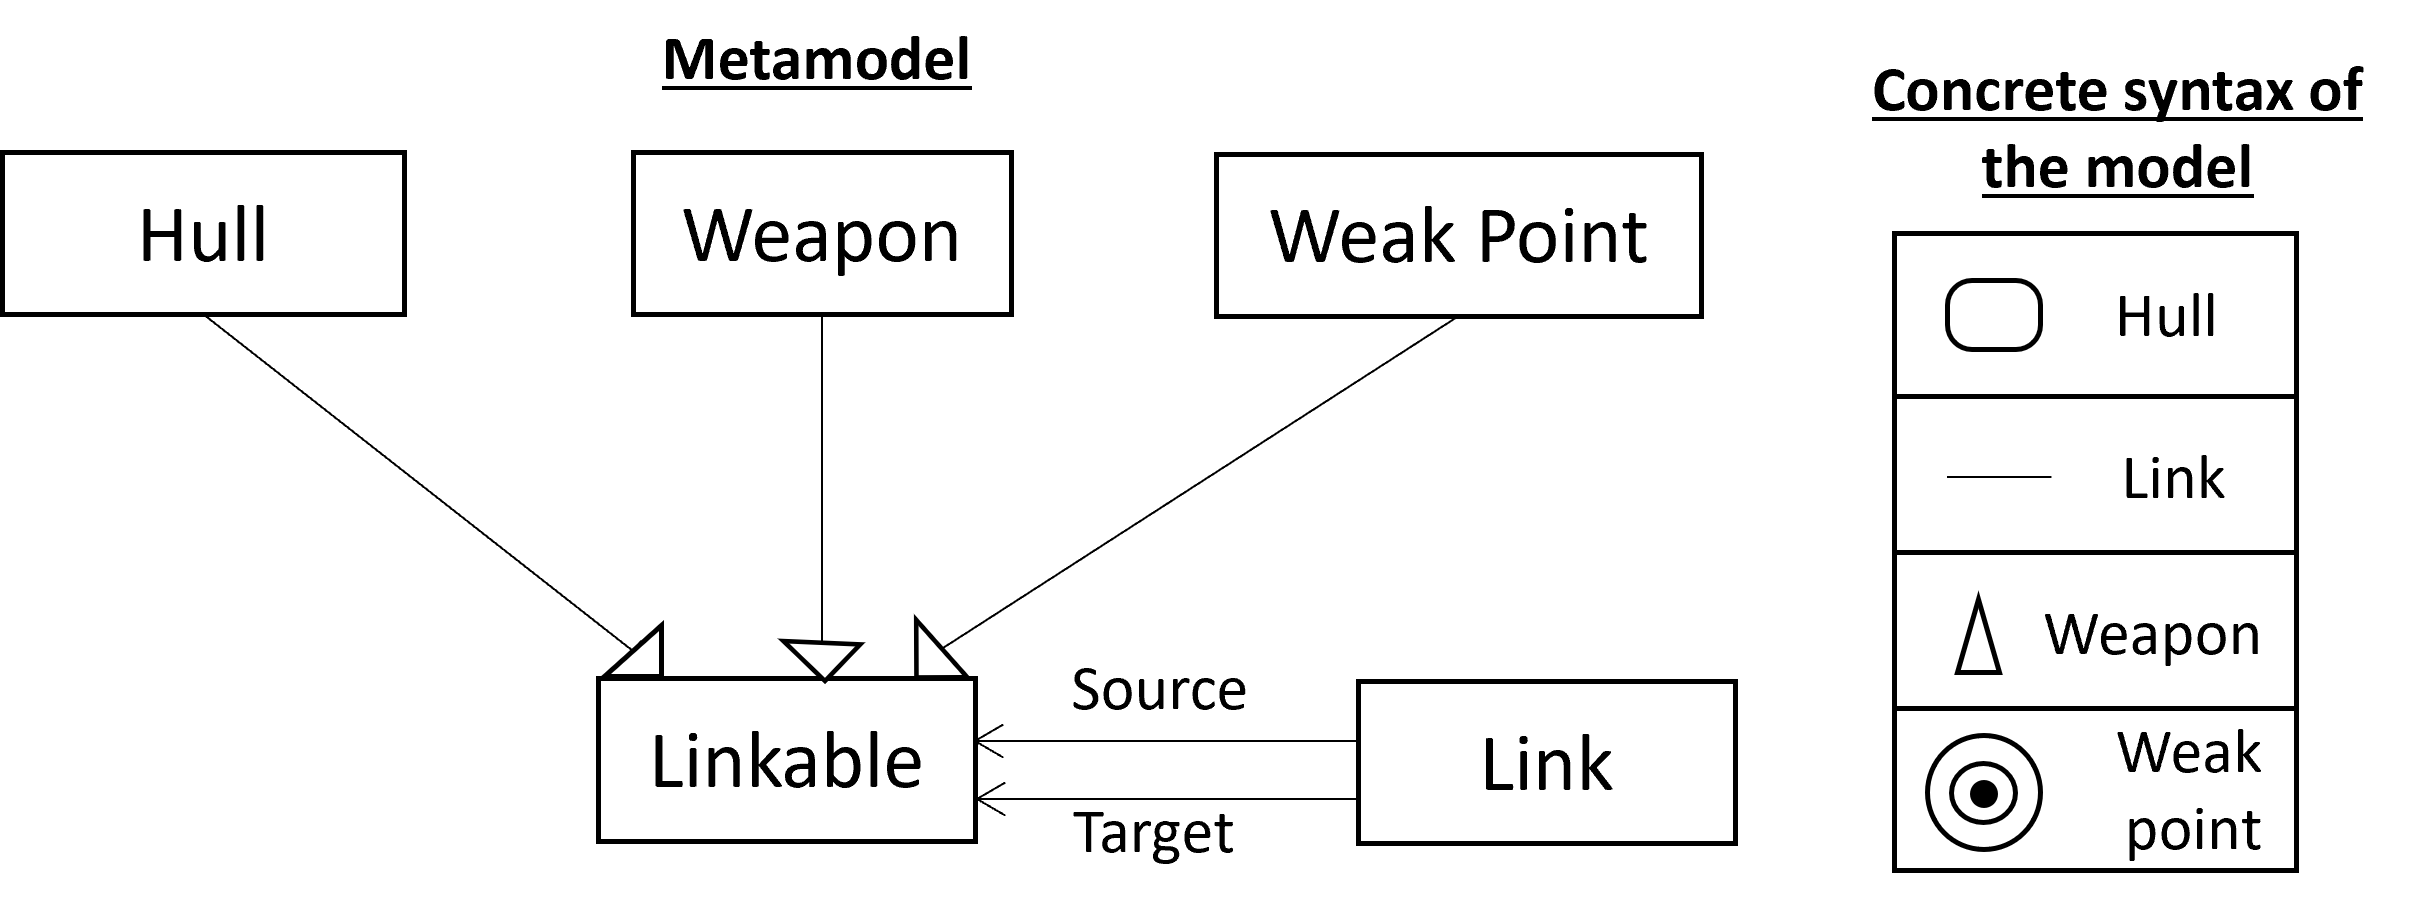
\includegraphics[width=0.35\textwidth]{Figures/metamodel+syntax.png}
    \caption{Simplified metamodel with the corresponding concrete syntax of the model.}
    \label{fig:metamodel+syntax}
\end{figure}

In the running example, the source donor model is a simplified version of an original \sq{boss} from \CaseStudy{}, called \sq{Serpent}. Fig.~\ref{fig:donor} shows the graphical representation of the donor model, differentiating each element of the model with a letter from A to S. It also shows with dashed lines the elements selected as organ (the elements H, I, J, K, N, O, P, Q).
This simplified example is inspired by the boss shown in Fig.~\ref{fig:scenario} with letter B. In the running example, the host is a model of a regular enemy that could appear in \CaseStudy{}. Fig.~\ref{fig:host} shows the graphical representation of the host model.

\begin{figure}[h]
    \centering
    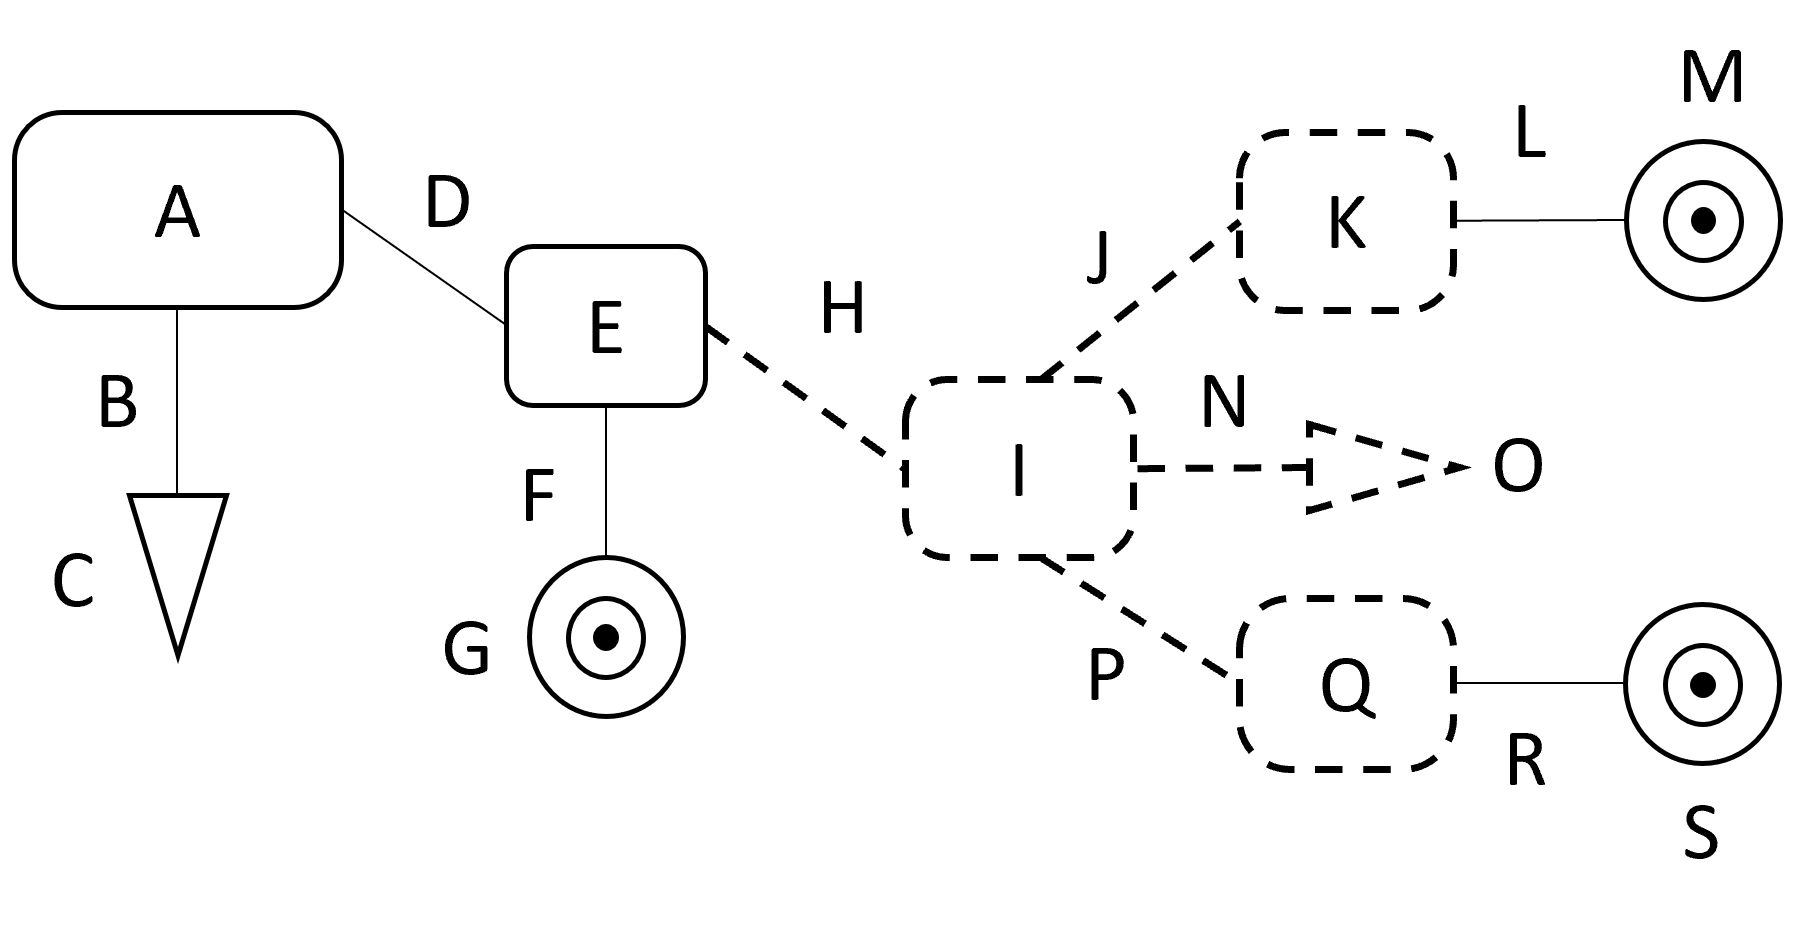
\includegraphics[width=0.35\textwidth]{Figures/donor+organ.png}
    \caption{Donor model with organ selection in dashed lines.}
    \label{fig:donor}
\end{figure}

\begin{figure}[h]
    \centering
    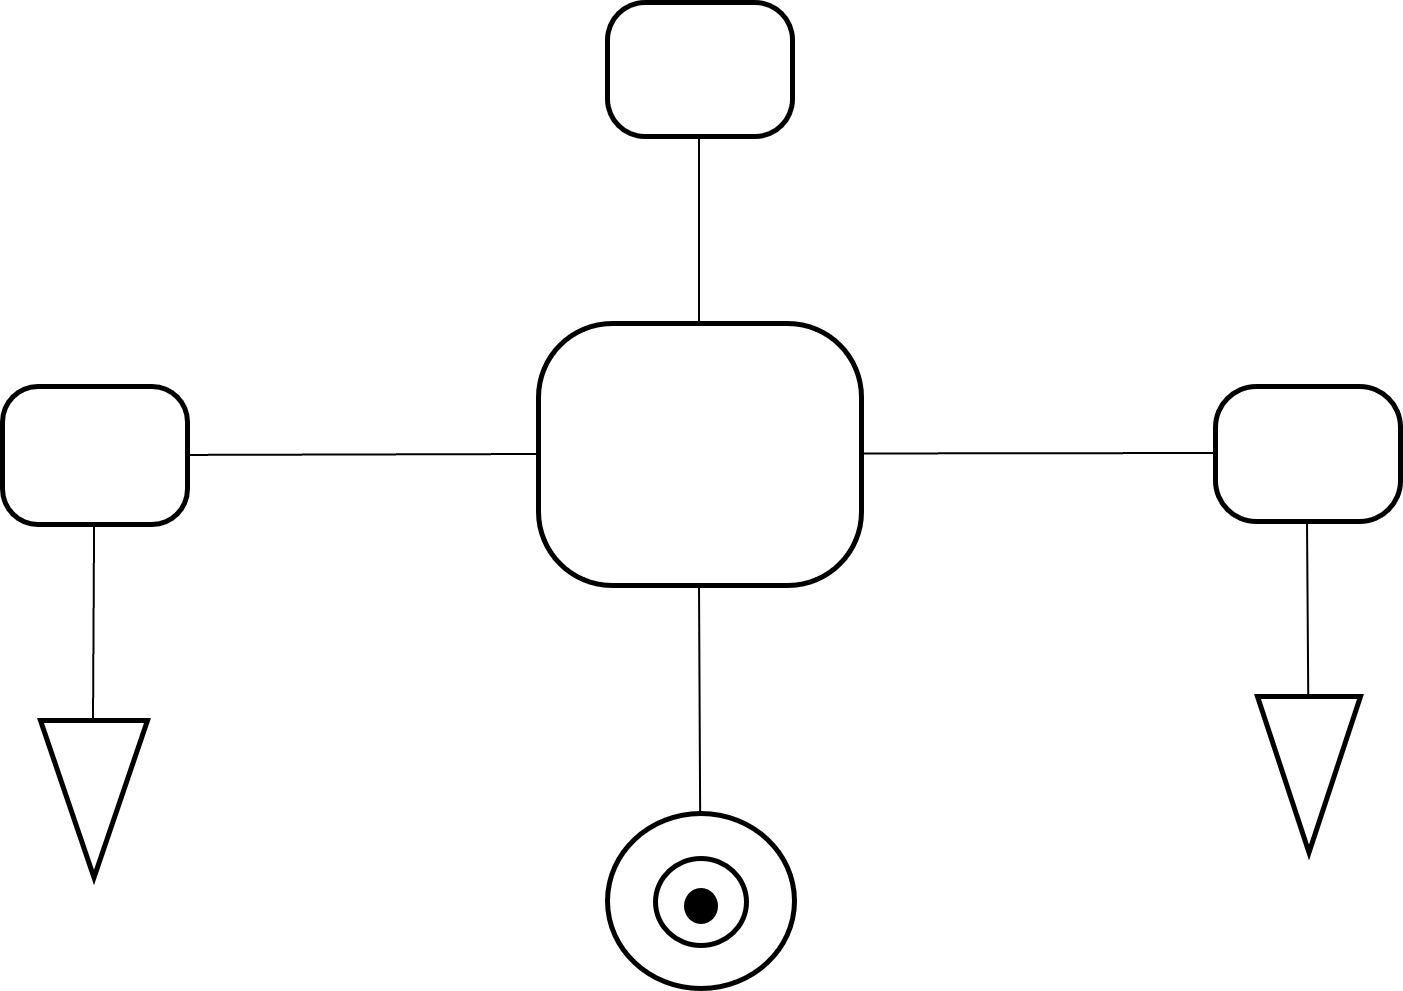
\includegraphics[width=0.2\textwidth]{Figures/host.png}
    \caption{Host}
    \label{fig:host}
\end{figure}

\subsection{Boundary detection}

To transplant an organ into a host we need to find a way to connect them. To do that we use the boundaries between the model elements of the organ and the host. A boundary is a connection point capable of connecting two distinct model elements within a model. The connection is restricted by the rules of the metamodel. In the simplified example in Fig.~\ref{fig:metamodel+syntax}, the Source and Target meta-relationships are the boundaries between the model elements of the models conforming to that metamodel. In other metamodel languages, there will be other meta-relationships with other names that will be the boundaries.

Imhotep automatically identifies the boundaries of the selected organ, and all the boundaries of the host. In the running example, the boundaries of the organ are the connection points between donor and host. The elements that connect with the rest of the donor are H, K, and Q. Fig.~\ref{fig:org_bound} shows the donor, the organ, and the boundaries (boundaries are represented by a circle crossed). The boundaries of the organ are as follows: b11 for the H element; b16 for the K element, and b25 for the Q element.

\begin{figure}[h]
    \centering
    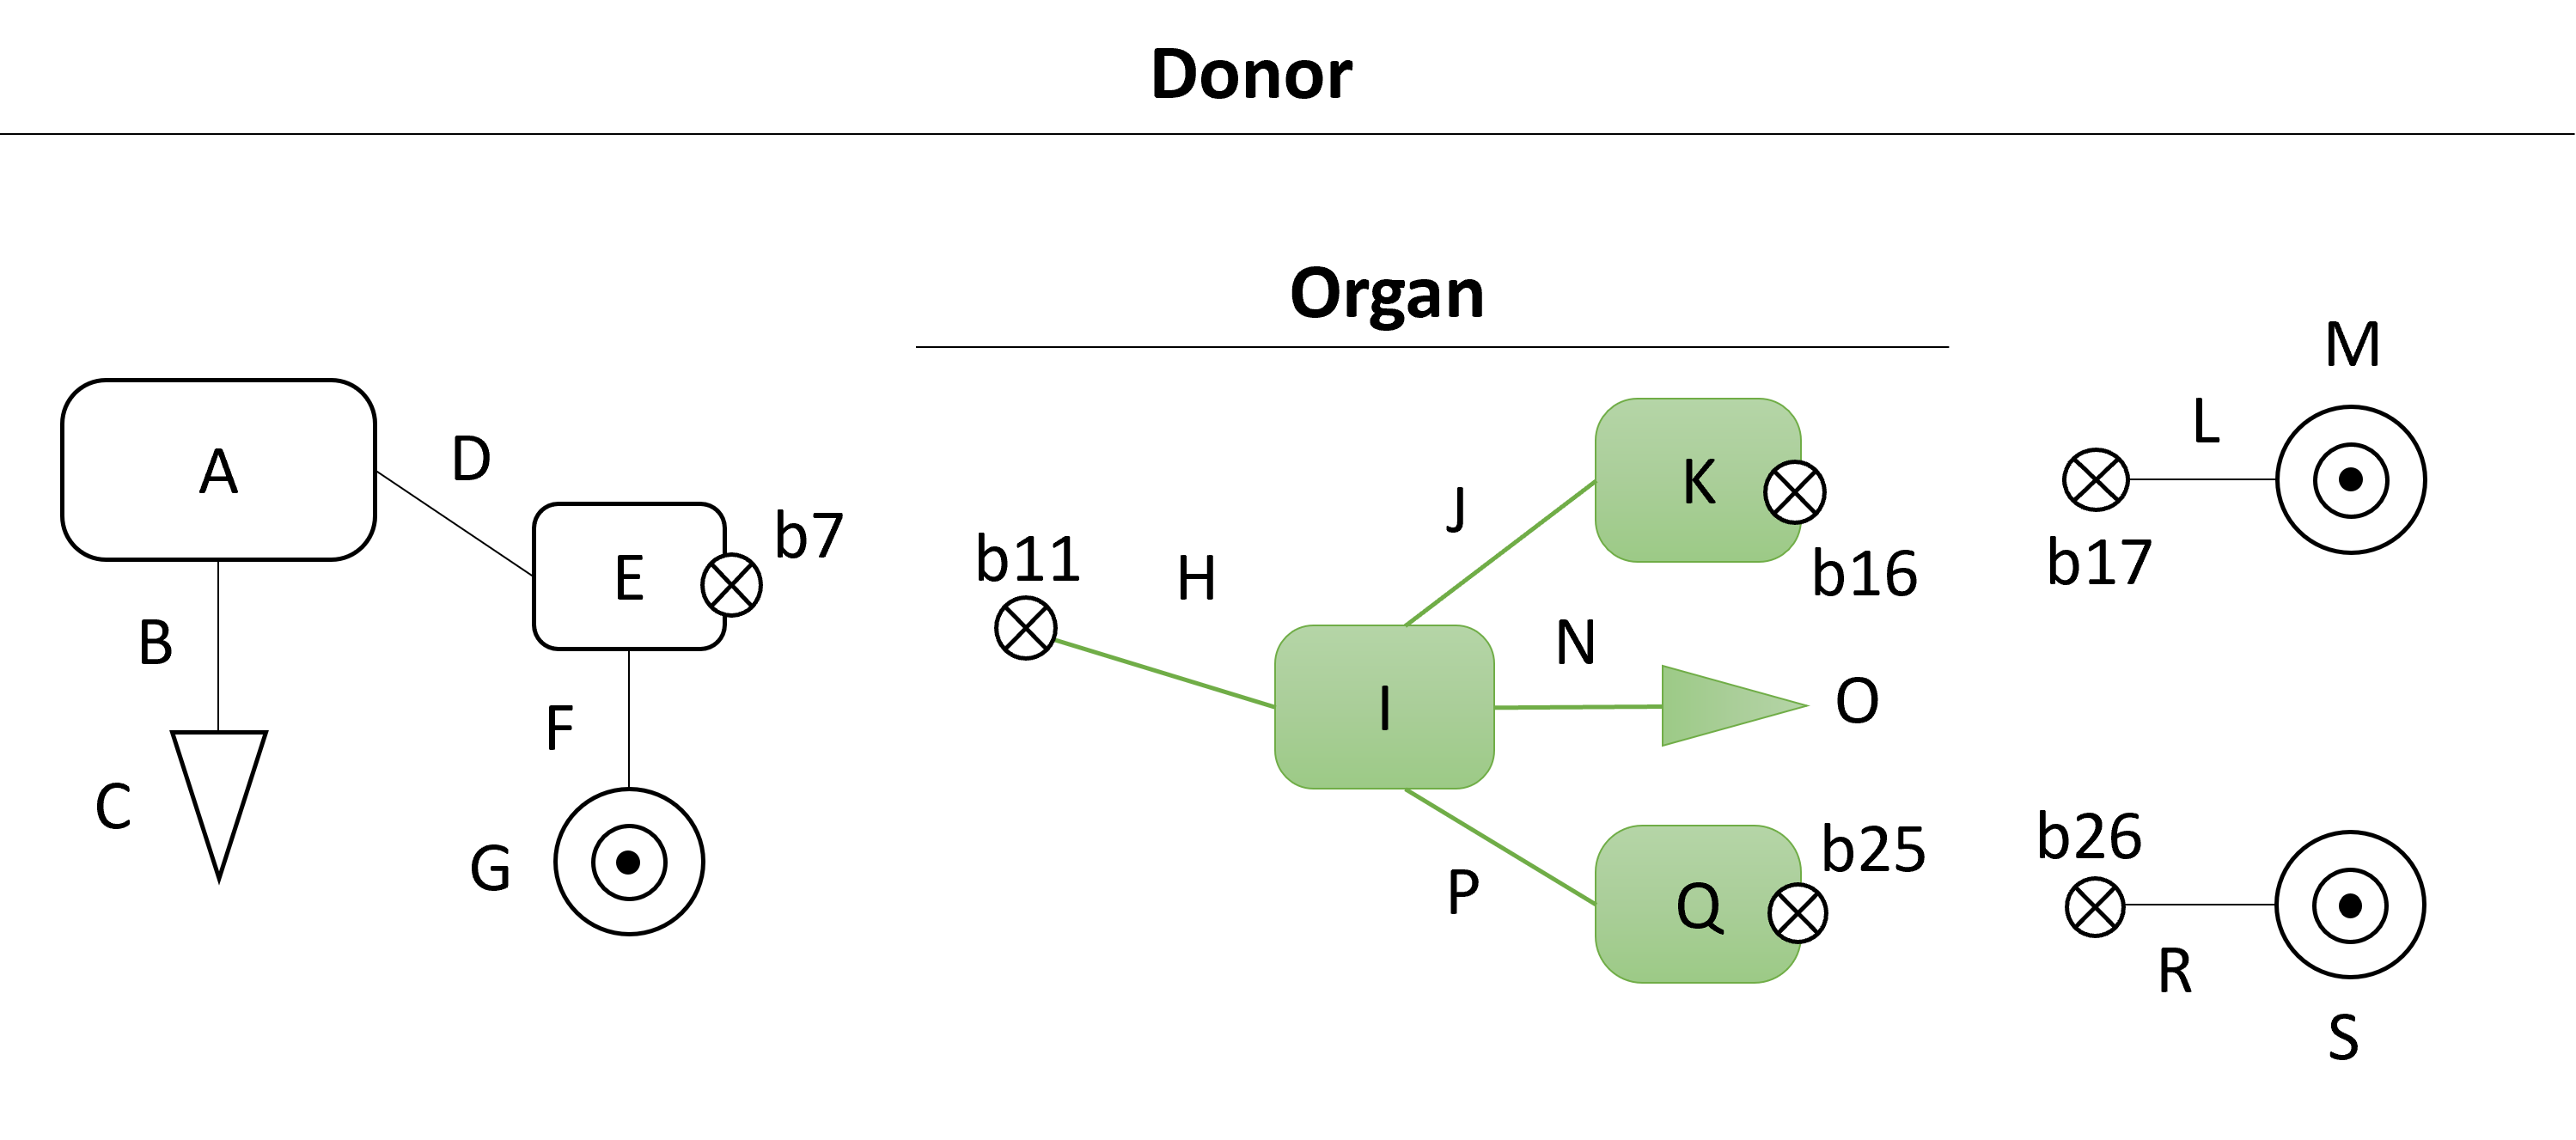
\includegraphics[width=0.45\textwidth]{Figures/donor+organ_boundaries.png}
    \caption{Donor model boundaries. The boundary is represented by a circle crossed.}
    \label{fig:org_bound}
\end{figure}

On the other hand, the boundaries of the host are all the points where its model elements connect. Figure~\ref{fig:host_bound} shows all the boundaries of the host of the running example. The host has a total of 19 boundaries identified by a tag from ba to bs.

\begin{figure}[h]
    \centering
    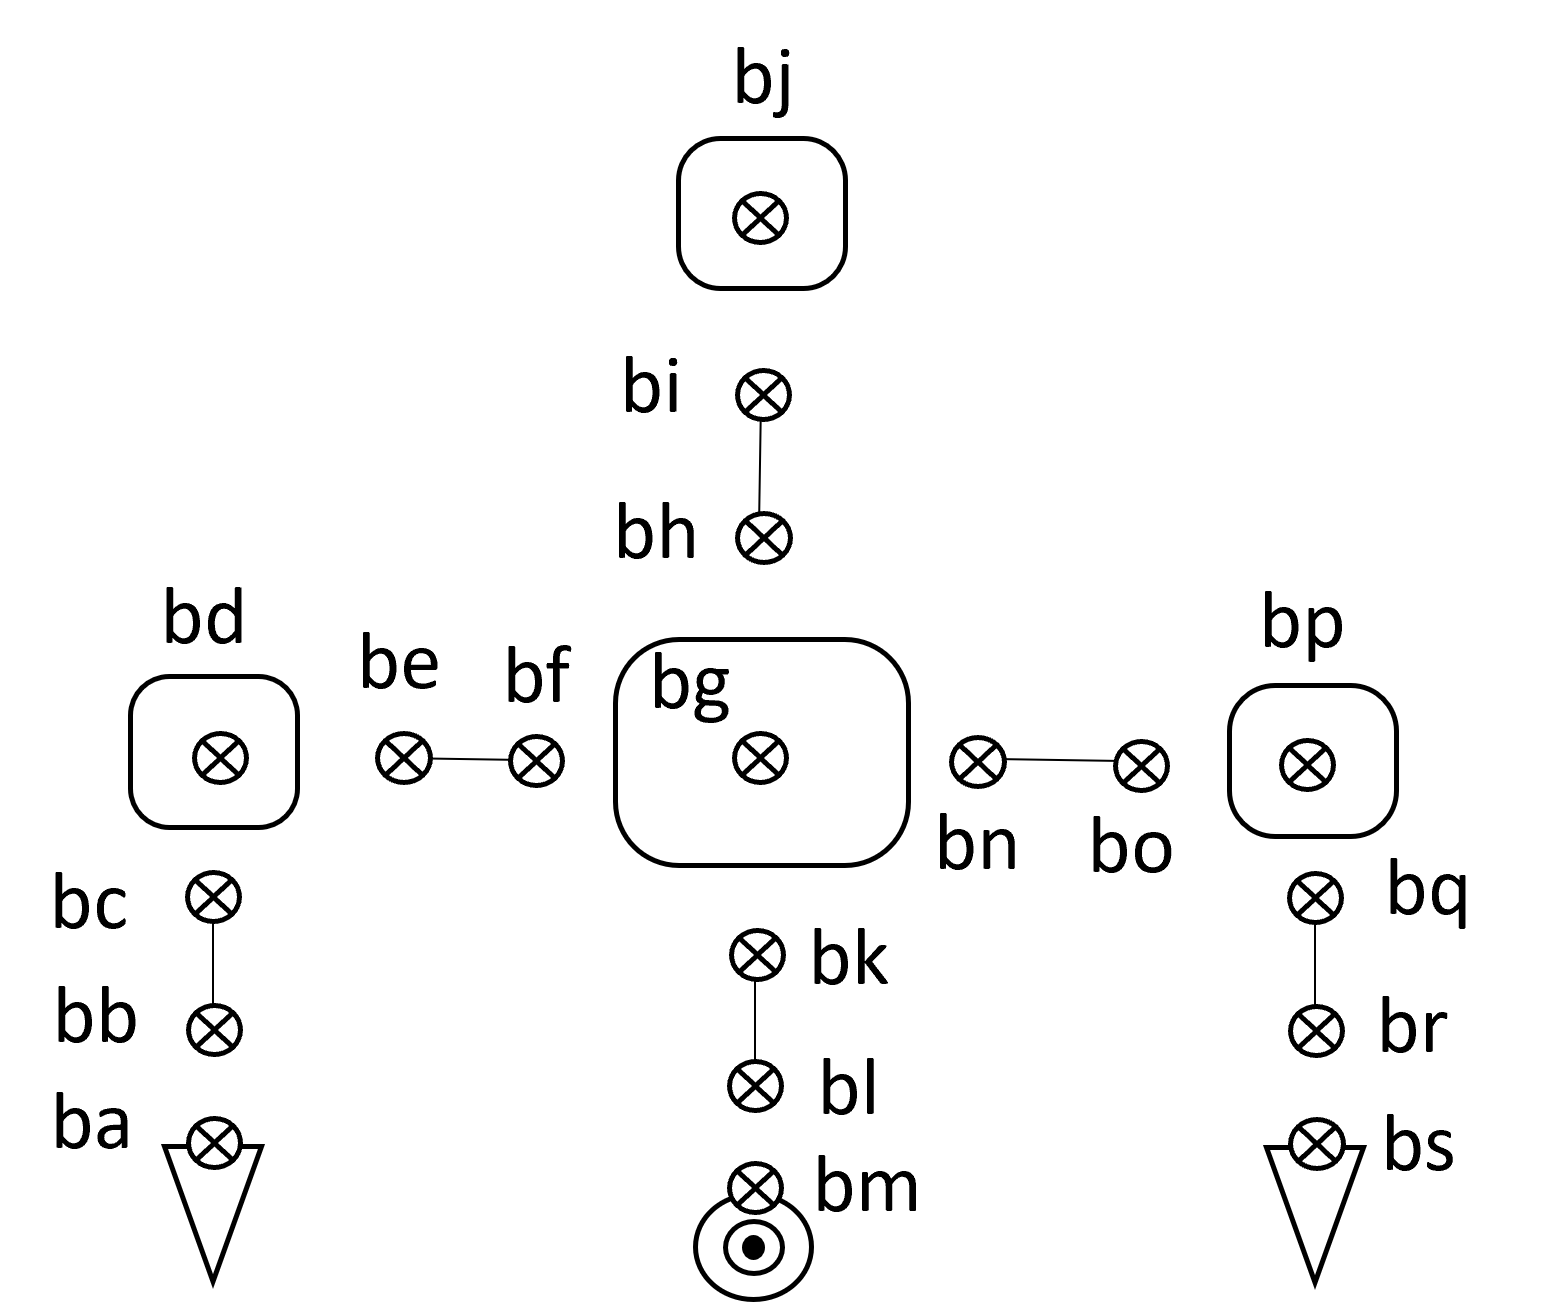
\includegraphics[width=0.35\textwidth]{Figures/host_boundaries.png}
    \caption{Host model boundaries. The boundary is represented by a circle crossed.}
    \label{fig:host_bound}
\end{figure}

\subsection{Boundary mapping}

In the boundary mapping step, \ApproachName{} determines the mapping between the boundaries of the organ and the host. For each boundary in the organ, Imhotep considers all compatible boundaries of the host, including the possibility of not connecting the boundary to the host boundaries. The boundary compatibility is determined by the metamodel.

Table~\ref{tab:boundaries} shows a boundary mapping between the organ and the host of the running example. The boundary b11 is a boundary from a \sq{Link} from the model and according to the metamodel it can connect to any \sq{Hull}, \sq{Weapon}, \sq{Weak Point}. The boundaries b16 and b25 are both \sq{Hulls} and they can connect with any \sq{Link}.

\begin{table}[h]
\centering
\resizebox{0.35\textwidth}{!}{
\begin{tabular}{|c|ll|}
\hline
{Organ boundaries} & \multicolumn{2}{c|}{{ \begin{tabular}[c]{@{}c@{}}Host \\      boundaries\end{tabular}}} \\ \hline
& \multicolumn{1}{c|}{ba} & \multicolumn{1}{c|}{bm} \\ \cline{2-3} 
& \multicolumn{1}{c|}{bd} & \multicolumn{1}{c|}{bp} \\ \cline{2-3} 
& \multicolumn{1}{c|}{bg} & \multicolumn{1}{c|}{bs} \\ \cline{2-3} 
\multirow{-4}{*}{b11} 
& \multicolumn{1}{c|}{bj} & \multicolumn{1}{c|}{Not connected} \\ \hline
& \multicolumn{1}{c|}{bb} & \multicolumn{1}{c|}{bc} \\ \cline{2-3} 
& \multicolumn{1}{c|}{be} & \multicolumn{1}{c|}{bf} \\ \cline{2-3} 
& \multicolumn{1}{c|}{bh} & \multicolumn{1}{c|}{bi} \\ \cline{2-3} 
& \multicolumn{1}{c|}{bk} & \multicolumn{1}{c|}{bl} \\ \cline{2-3} 
& \multicolumn{1}{c|}{bn} & \multicolumn{1}{c|}{bo} \\ \cline{2-3} 
\multirow{-6}{*}{\begin{tabular}[c]{@{}c@{}}b16\\    \\ b25\end{tabular}} 
& \multicolumn{2}{c|}{Not connected} \\ \hline
\end{tabular}}
\caption{Mapping  of compatible boundaries between organ and host.}
\label{tab:boundaries}
\end{table}

\subsection{Initialize population}

In evolutionary algorithms a population is a collection of possible solutions for a problem.
The encoding is the problem representation that an algorithm is capable to understand. 

In our work, the encoding requires a binary vector that represents the organ in the donor, and the boundary mapping (see Fig.~\ref{fig:encoding}). In the binary vector, each element from the model is a position from the vector. If a position in the vector has a \sq{1}, it means that the element from the model is part of the organ. On the other hand, each boundary from the organ gets assigned a compatible boundary from the host.
%In our work, each individual represents a software model from the game. We use a similar encoding version of Blasco \etal~\cite{blasco2021evolutionary} that has been adapted to work with transplantations. The size of the encoding in the previous work was 64 and in this work its size is of 150.
The initial population of Imhotep contains individuals composed by the host and the organ placed in a random position (a random mapping between the organ boundaries and the compatible organ boundaries).

\begin{figure}[h]
    \centering
    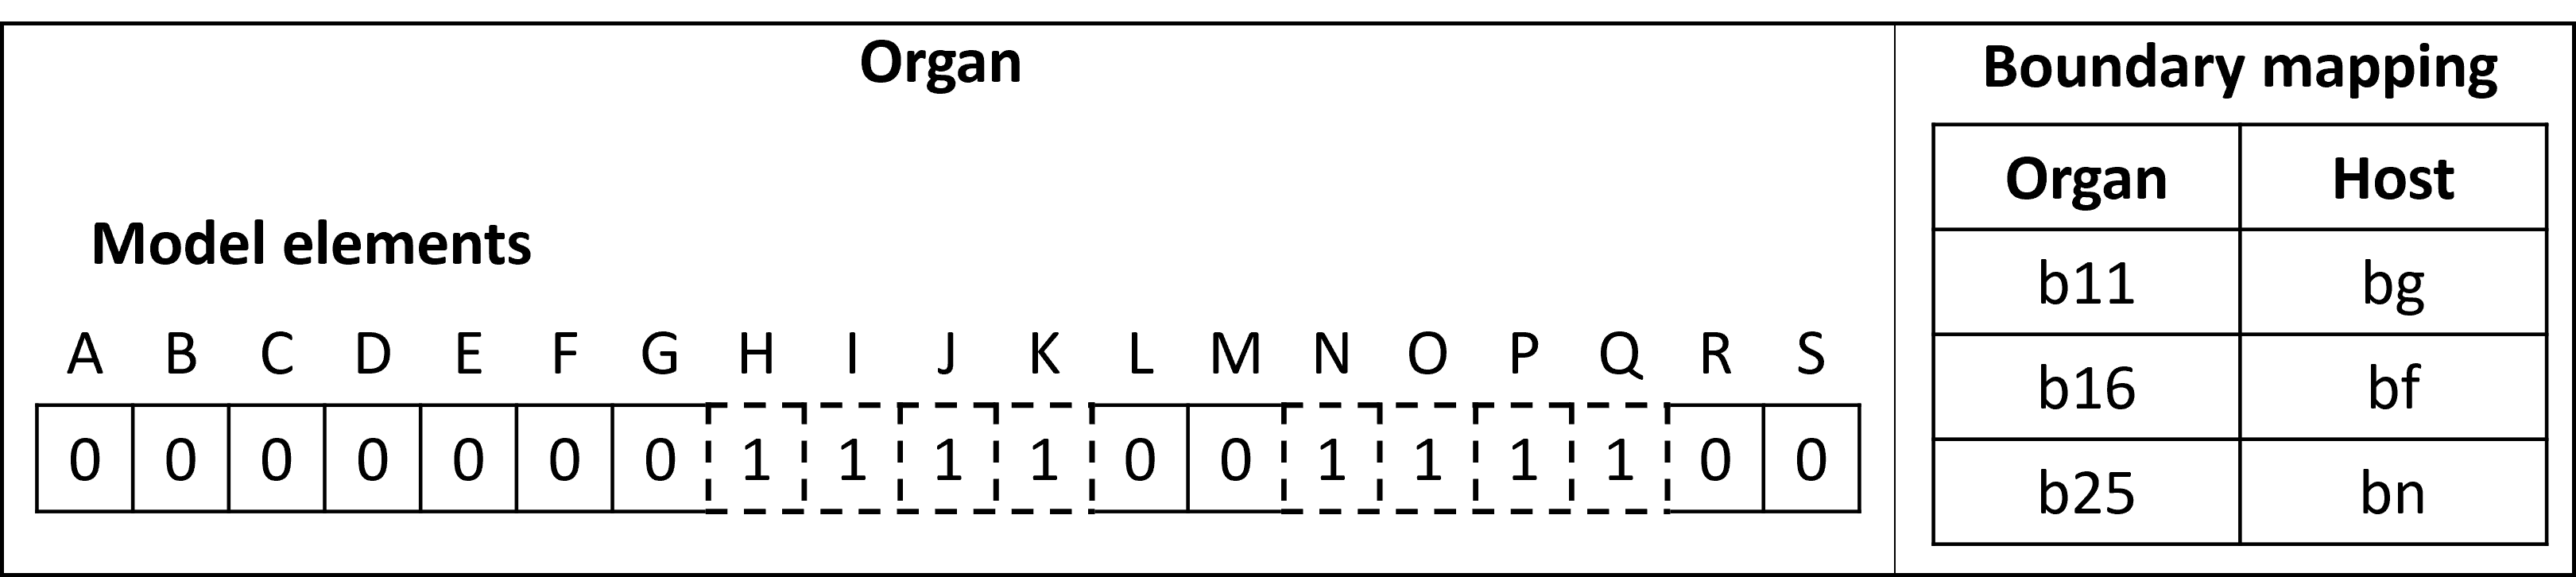
\includegraphics[width=0.48\textwidth]{Figures/encoding.png}
    \caption{Example of encoding.}
    \label{fig:encoding}
\end{figure}

\subsection{Genetic Operators}

Imhotep has genetic operations (selection, crossover, and mutation) to generate new individuals of the population. To select the individuals, we use the ranking selection, which ranks the population by the objective function and takes the top individuals in the current population.

We use a single, random, cut-point crossover. It starts by selecting and splitting two parent solutions at random. When two parent individuals are selected, a random cut point is determined to split them into two sub-vectors.
Then, the crossover creates two child solutions by putting the first part of the first parent with the second part of the second parent for the first child and putting the first part of the second parent with the second part of the first parent for the second child.
Finally, the new individual has a probability to mutate any value of the encoding. 

Fig.~\ref{fig:candidates} shows example of new individuals that could results from the running example. For simplicity, these individuals have unaltered organs but illustrate different boundary mappings between organ and host.

\begin{figure}[h]
    \centering
    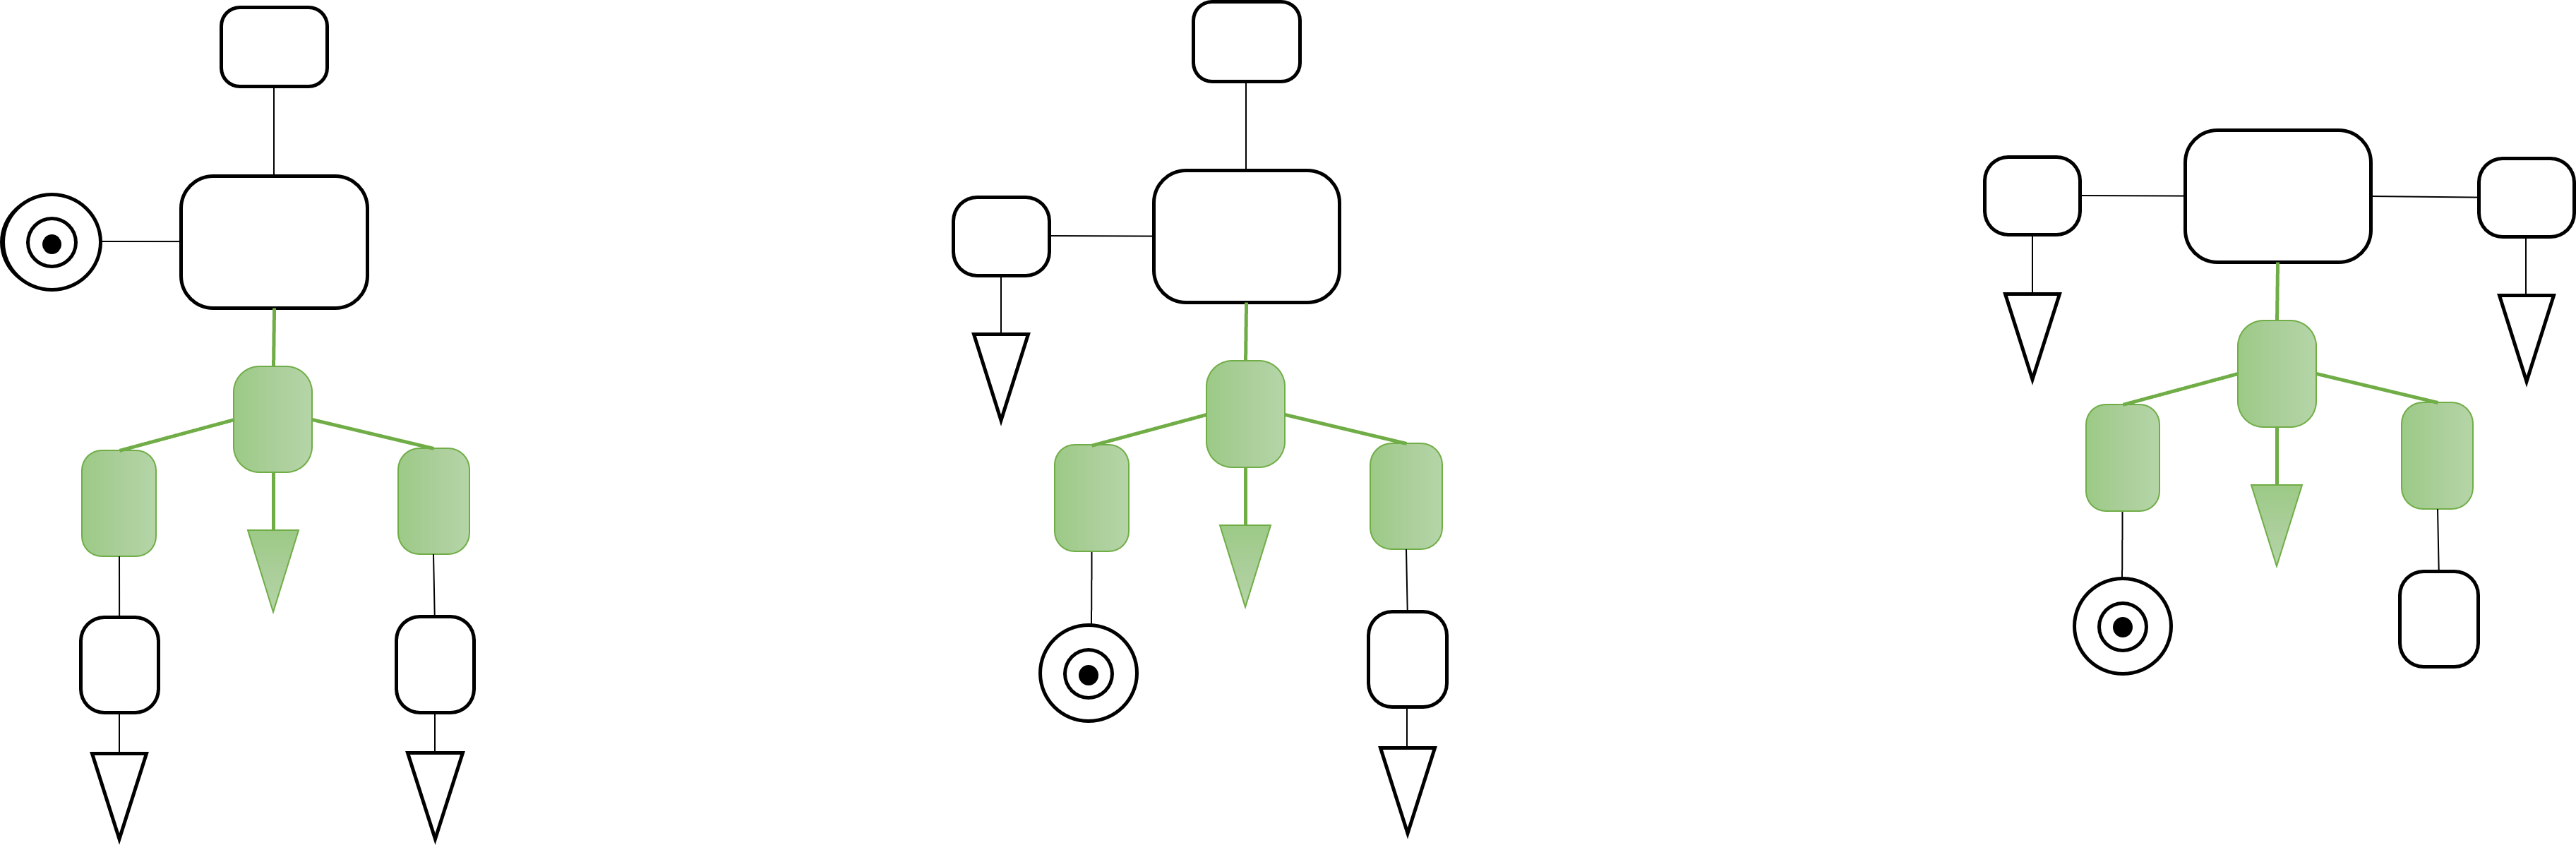
\includegraphics[width=0.45\textwidth]{Figures/candidates.png}
    \caption{Example of individuals.}
    \label{fig:candidates}
\end{figure}

\subsection{Objective function}

Our work proposes to harness video games' NPCs to run simulations that provide data to assess the transplantations. The first thing that differentiates video games from traditional software is that the basic requirement of video games is \sq{fun}. \sq{Fun} is an abstract concept and the developers are in charge of interpreting it. In fact, different developers may have different interpretations. For some game developers, \sq{fun} is achieved with a difficult game that is very rewarding when progress is made (e.g., Dark Souls). While for other developers, \sq{fun} is achieved by effortlessly killing enemies (e.g., Dynasty Warriors). Therefore, we argue that the developer intent is key for content generation.

Specifically, we propose to introduce the generated content (each individual in the population) into a simulation of the video game. The simulation produces a data trace of the events that have occurred. Using the data from the trace, we can check how well aligned are the events with the intention of the developers. In the running example, the simulation is a duel between a spaceship and a boss. The simulation generates data about the duel, such as the damage inflicted. The intention of the developers may be that the duel ends with the victory of the spaceship with a remaining life of less than 10\%.

Our proposal does not require ad hoc development of simulations. We propose that the simulations leverage mainly the NPCs (but also more video game elements, such as scenarios or items like weapons or powerups). NPCs are naturally developed during the development process of a video game. In other words, NPCs are integral components of  most video game genres such as First-Person Shooter (FPS), Real-Time Strategy (RTS), our racing games. We aim two goals with the aforementioned. On the one hand, it makes the use of simulations cheaper, i.e. it does not involve additional development costs, and secondly, it facilitates fidelity to the video game compared to ad hoc development. In the running example, during the simulation, the generated content is the boss, who can be accompanied by more NPCs acting as secondary enemies. Additionally, the spaceship that confronts the boss is a NPC representing an allied ship. Finally, the scenario, and items such as weapons or powerups also belong to the game itself.

In this work, the Simulation-based variant of \ApproachName{} assesses the transplants through a simulation of a game battle between the boss (Host') and a NPC spaceship. The information retrieved from the simulation is the data that the developers regard as relevant, using their domain knowledge. Hence, our approach takes into account  the percentage of simulated player victories ($F_{Victory}$) and the percentage of simulated player health left once the player wins a duel ($F_{Health}$).
The calculation of $F_{Victory}$ and $F_{Health}$ is performed in the same
way as Blasco \etal~\cite{blasco2021evolutionary}:

$F_{Victory}$ is calculated as the difference between the number of human player victories ($V_{P}$) and the optimal number of victories (33\%, according to the developers of \CaseStudy{} and their criteria) ($V_{Optimal}$):
\begin{equation}
F_{Victory} = 1 -\frac{\mid V_{Optimal} - V_{P} \mid}{ V_{Optimal}}
\end{equation}

$F_{Health}$, which refers to completed duels that end in spaceship victories, is the average difference between the spaceship's health percentage once the duel is over ($\Theta_{P}$) and the optimal health level that the spaceship should have at that point ($\Theta_{Optimal}$, 20\%, according to the developers):
\begin{equation}
F_{Health} = 1 - \frac{\sum\limits_{d=1}^{V_{P}}\frac{\mid \Theta_{Optimal} - \Theta_{P} \mid}{ \Theta_{Optimal}}}{V_{P}}
\end{equation}

$F_{Overall}$ is an average fitness value for a boss model that includes the fitness criteria described above. FOverall also includes a validation part. The validation part is to avoid models with inconsistencies. The validity of the models is performed by a run-time interpreter that is part of the game. When the model is stated as non-valid the value of Validity will be 0. $F_{Overall}$ can assume a value in [0, 1] which is used to assess a boss model when our \ApproachName{} approach is applied to the \CaseStudy{} case study.

\begin{equation}
F_{Overall} = min( Validity, \frac{\sum\limits_{i=1}^{N}F_{i}}{N} )
\end{equation}


% The objective function in \ApproachName{} assesses the quality of each individual as a model. First, as done in previous work that use \CaseStudy{}~\cite{blasco2021evolutionary}, the models pass through a validation process followed by a quantitative measurement. In our work we assess quantitatively the objective function by two means: Test-based and Simulation-based objective functions. We use two different objective functions due to the differences in the the state-of-the-art of software transplantation and PCG. The state-of-the-art in software transplantation mainly work with Test-based objective function, while the state-of-the-art in NPCs PCG work with Simulation-based objective function.

% The validation step before the Test-based or Simulation objective function is a requirement that \CaseStudy{} integrates in the game to avoid models with inconsistent data. The validity of the models is performed by a run-time interpreter that is part of the game. When the model is stated as non-valid the value of the objective function will be 0.0.

% The models that pass the validation process will then be assess by the Test-based and Simulation-based objective functions.
% For the Test-based objective function we ask the developers to provide the set of tests that they consider relevant to our work. The developers from \CaseStudy{} provided us with a total of 243 tests selected based on their domain knowledge. The objective value will be retrieved when each individual pass through the 243 tests, normalized in a scale of [0, 1]. An individual which passes the 243 tests will obtain 1.0, on the contrary if it does not pass any test it will obtain 0.0.

% On the other hand, the Simulation-based objective function as in Blasco \etal~\cite{blasco2021evolutionary} simulates an in game battle between the boss and a player. The information retrieved from the simulation is the data that the developers regard as relevant, using their domain knowledge. Hence, our approach takes into account the percentage of simulated player victories ($F_{Victory}$) and the percentage of simulated player health left once the player wins a duel ($F_{Health}$).
% The calculation of $F_{Victory}$ and $F_{Health}$ is performed in the same
% way as Blasco \etal~\cite{blasco2021evolutionary}:

% $F_{Victory}$ is calculated as the difference between the number of human player victories ($V_{P}$) and the optimal number of victories (33\%, according to the developers of \CaseStudy{} and their criteria) ($V_{Optimal}$):
% \begin{equation}
% F_{Victory} = 1 -\frac{\mid V_{Optimal} - V_{P} \mid}{ V_{Optimal}}
% \end{equation}

% $F_{Health}$, which refers to completed duels that end in human player victories, is the average difference between the human player's health percentage once the duel is over ($\Theta_{P}$) and the optimal health level that the player should have at that point ($\Theta_{Optimal}$, 20\%, according to the developers):
% \begin{equation}
% F_{Health} = 1 - \frac{\sum\limits_{d=1}^{V_{P}}\frac{\mid \Theta_{Optimal} - \Theta_{P} \mid}{ \Theta_{Optimal}}}{V_{P}}
% \end{equation}

% $F_{Overall}$ is an average fitness value for a boss model that includes the fitness criteria described above. $F_{Overall}$ can assume a value in [0, 1] which is used to assess a boss model when our \ApproachName{} approach is applied to the \CaseStudy{} case study.

% \begin{equation}
% F_{Overall} = min( Validity, \frac{\sum\limits_{i=1}^{N}F_{i}}{N} )
% \end{equation}
